% \documentclass[]{article}
% \documentclass[onecolumn]{IEEEtran}
% onecolumn for readability
\documentclass[]{IEEEtran}

% -----------------------------------------------------
% Preamble
% -----------------------------------------------------
% Math Packages
\usepackage{physics}
\usepackage{amsmath, amssymb, empheq}
\usepackage{thmtools}
% \usepackage[per-mode=symbol]{siunitx}

% Format Packages/Settings
\usepackage{todonotes}
% \usepackage[disable]{todonotes}
\usepackage{xcolor}
\usepackage[]{hyperref}
\renewcommand{\figureautorefname}{Fig.}
% \usepackage[inline, shortlabels]{enumitem}
\usepackage{paralist}
\usepackage{cite}
\usepackage{graphicx}
\usepackage{wrapfig}

% Theorems
\newtheorem{definition}{Definition}
\newtheorem{theorem}{Theorem}
\newtheorem{lemma}{Lemma}
\newtheorem{corollary}{Corollary}
\newtheorem{remark}{Remark}
\newtheorem{system}{System}

% % Custom Commands
% \newcommand{\R}{\mathbb{R}}
% \newcommand{\N}{\mathbb{N}}
% \newcommand{\st}{ \ | \ }

% \newcommand{\E}{\mathcal{E}}
% \newcommand{\Ebar}{\bar{\mathcal{E}}}
% \newcommand{\X}{\mathcal{X}}
% \newcommand{\Xbar}{\bar{\mathcal{X}}}
% % \newcommand{\U}{\mathcal{U}}
% % \newcommand{\Ubar}{\bar{\mathcal{U}}}
% \newcommand{\F}{\mathcal{F}}


%% Title and stuff
\title{
    Path Planning for Autonomous Vehicles based on Nonlinear MPC with using a 3DOF Kinematic Bicycle Model
}
\author{
    Jonas Wagner

    \thanks{

        The author is with the Mechanical Engineering Department at the University of Texas at Dallas, Richardson, TX, USA 
        {\tt\small jonas.wagner@utdallas.edu}

        \begin{wrapfigure}{r}{0.15\columnwidth}
            
\includegraphics[width=0.15\columnwidth]{figs/NOVA-logo.png}
        \end{wrapfigure}
        
        Additional acknowledgements for this project for Jusin Ruths (research advisor) and Justin Koeln (course instructor).

        The future implementation of this work would not be possible without the work done by the amazing undergraduate students within the Nova Lab.
    }
}


% -----------------------------------------------------
% Begin Document
% -----------------------------------------------------
\begin{document}

% -----------------------------------------------------
% Title and Abstract
% -----------------------------------------------------
\maketitle
\begin{abstract}
    In this project, NOVA's autonomous vehicle, Hail Bopp, is modeled as a 3DOF Kinematic Bicycle Model and then used in a nonlinear MPC-based path-planning approach.
    The MPC solution is then used in a closed-loop simulation and the feasibility of the approach is explored.
\end{abstract}

% % -----------------------------------------------------
% % Introduction
% % -----------------------------------------------------
\section{Introduction}

Nova is UT Dallas's autonomous driving group that is run by undergrads as part of the Applied Systems Lab.
The objective for nova is to develop an open-source autonomous driving stack (Navigator) for use by researchers.
Specifically the Applied Systems Lab will eventually apply and test out the cyber-physical system security techniques and how they can be used on autonomous vehicles.\cite{nova}

\begin{figure}[h]
    \centering
    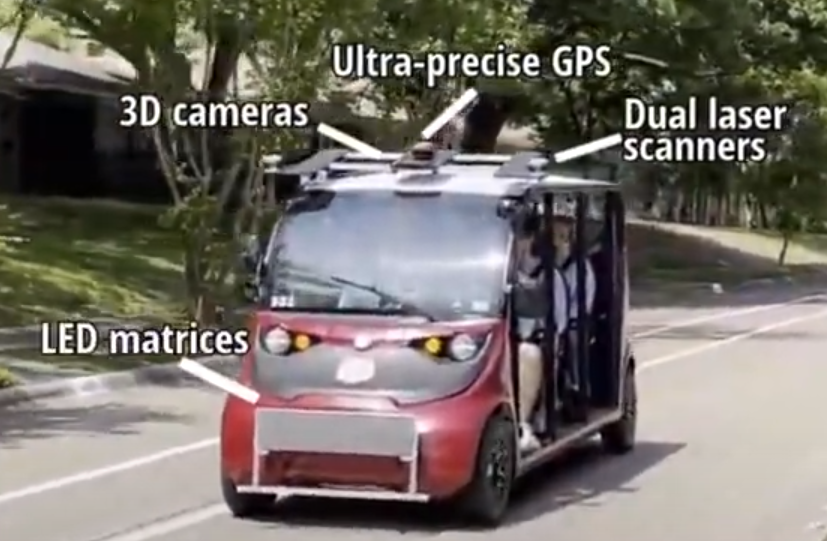
\includegraphics[width=0.7\columnwidth]{figs/NOVA-annotatedImage.png}
    \caption{Hail Bopp with labeled sensors.}
\label{fig:hailBopp}
\end{figure}

The primary vehicle used by Nova is Hail Bopp which is a Polaris Gem e6, seen in \autoref{fig:hailBopp}, and is modified to allow for autonomous operation.
There are many sensors added to the system (i.e. GPS, cameras, radar, lidar) that are then used in an entire perception stack to determine the current state of the vehicle and the surrounding environment.

The environment perception stack is shown operating on the simulated vehicle, done in CARLA\cite{carla,dosovitskiy2017carla}, along with the test run around campus in \autoref{fig:perceptionStack}.

\begin{figure}
    \centering
    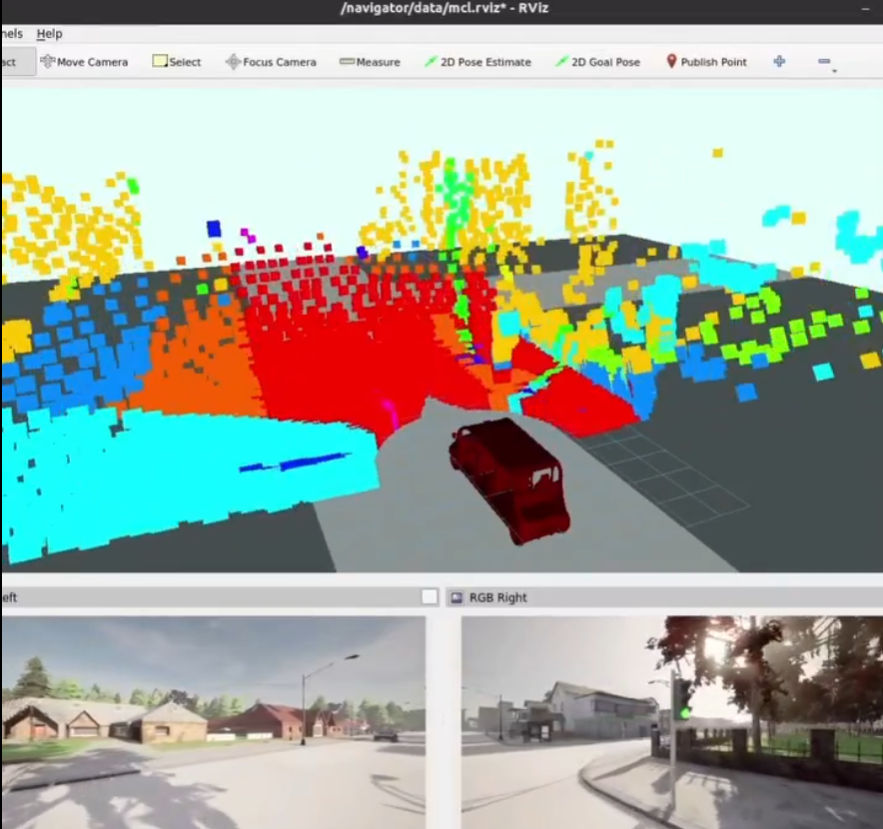
\includegraphics[width = 0.5 \columnwidth]{figs/NOVA-carla_screenshot.png}\\
    \vspace{0.5em}
    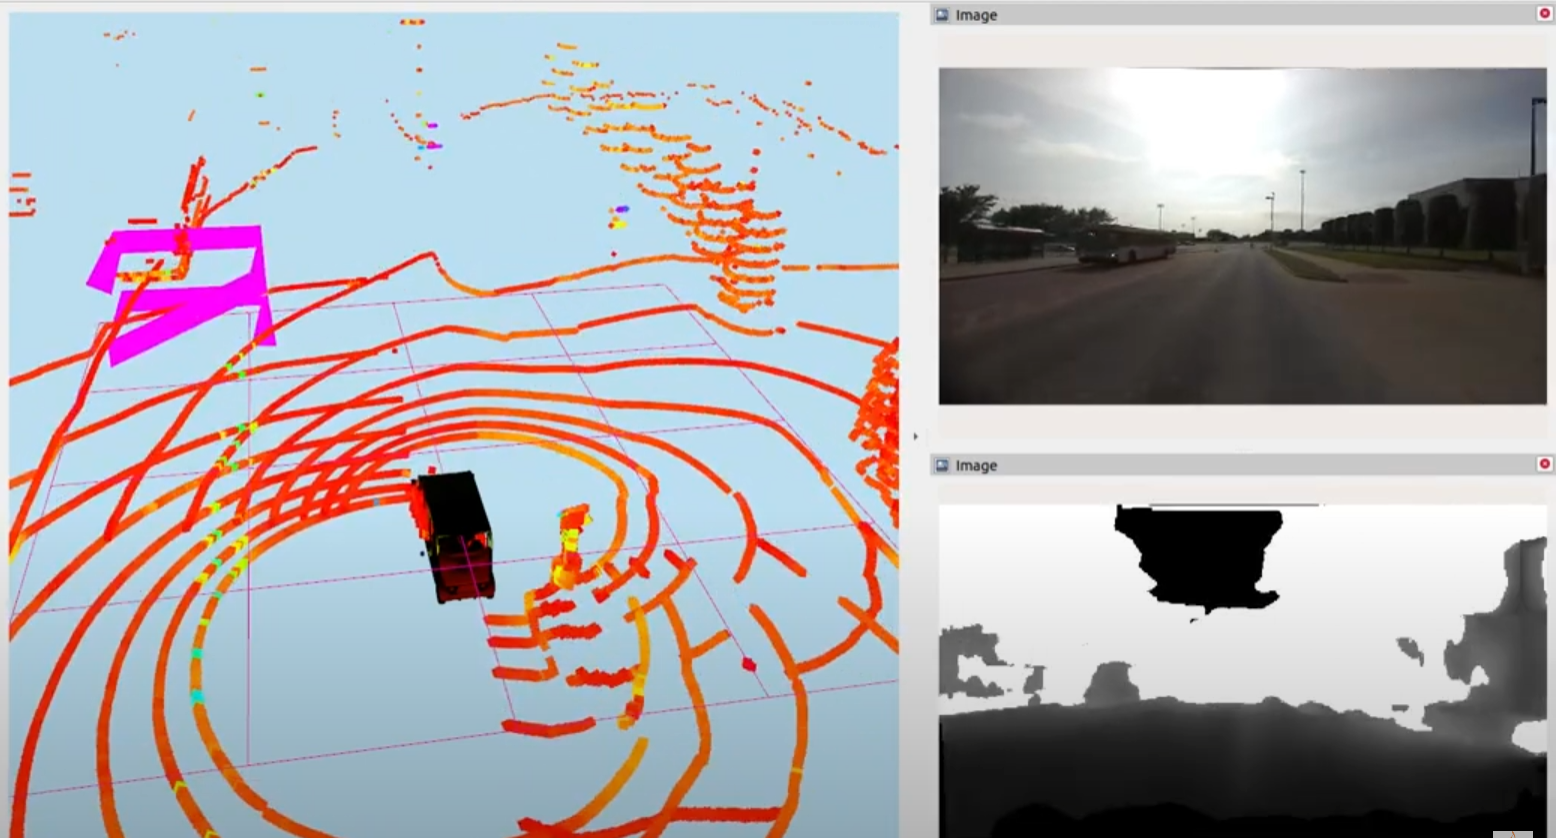
\includegraphics[width = 0.7 \columnwidth]{figs/NOVA-sensorData_screenshot.png}
    \caption{NOVA perception stack in operation within simulated environment (top) and around campus (bottum).}
\label{fig:perceptionStack}
\end{figure}

% -----------------------------------------------------
% Problem Definition
% -----------------------------------------------------
\section{Problem Definition}
\label{sec:pblm_def}
% Path Planning
\subsection{Path Planning}
\label{subsec:pathPlanning}

The objective of this project was to create high-fidelity MPC controller produce an optimal trajectory to reach a waypoint given the occupancy map of the environment.
This controller will then be used to generate training data for a neural network which will be able to perform an approximation of this controller in real-time.

From the perception stack, the current vehicle states (local and global) will be known to some uncertainty and the surrounding environment will be processed into a predicted occupancy map.
This occupancy map will be assumed to already have weights corresponding to where it is safe/ideal for the vehicle to be in the future.

% Model Definition
\subsection{Model Definition}
\subsubsection{3-DOF Bicycle Model}\label{subsec:mdl_def}
Hail-Bopp is considered to be a standard 4-wheel ackermann-steering vehicle
% , seen in \autoref{fig:ackermannModel}, 
whose approximation to a 3 degree of freedom bicycle model is detailed in\cite{casanova_thesis} and\cite{vehcileDynamics_chapter2a}.
A diagram of the bicycle model is shown in \autoref{fig:bikeModel_diagram}.
% \begin{figure}[h]
%     \centering
%     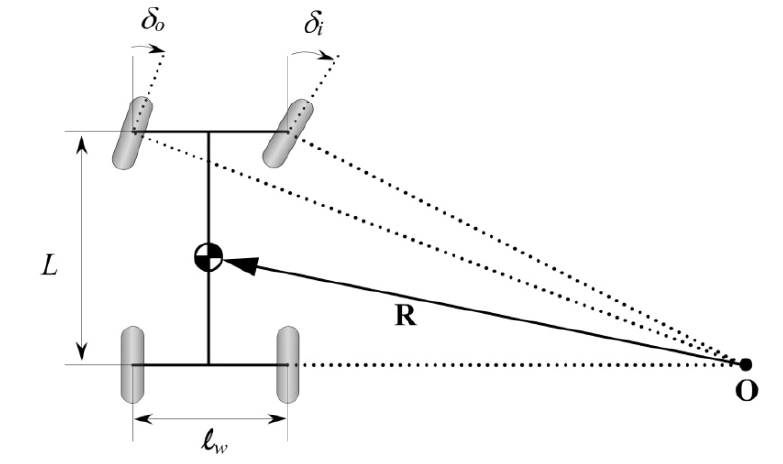
\includegraphics[width=0.7\columnwidth]{figs/ackermannModel.png}
%     \caption{ackermannn-steering vehicle model diagram.}
%\label{fig:ackermannModel}
% \end{figure}

\begin{figure}[h]
    \centering
    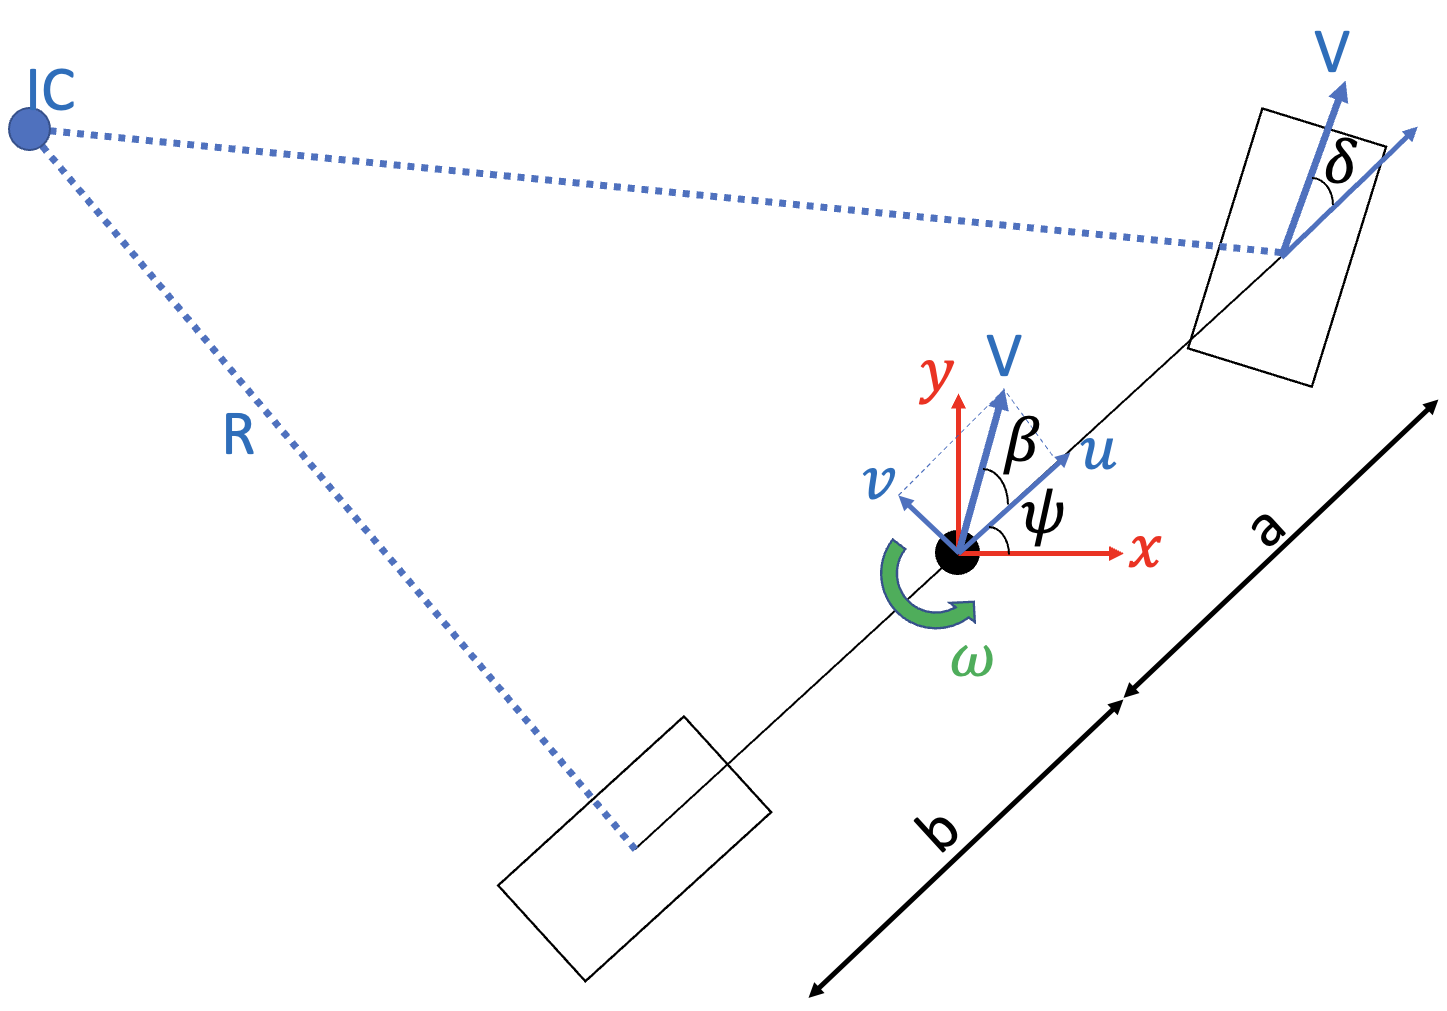
\includegraphics[width=0.9\columnwidth]{figs/BicycleModel.png}
    \caption{A diagram of the 3-dof bicycle model.}
\label{fig:bikeModel_diagram}
\end{figure}

Due to computation complexity, the kinematic model derivation is used which focuses solely on the relationship between the system inputs and outputs.
This does ignore some dynamics, namely the relationship between the actual forces and torques needed to induce vehicle movement, but still incorporates the important nonlinear relationships between steering angle and the vehicle rotation.

These simple kinematic model equations of motion are given in \eqref{eq:bikeModel}:
\begin{equation}\label{eq:bikeModel}
    \begin{cases}
        \dot{x} = V \cos(\psi + \beta)\\
        \dot{y} = V \sin(\psi + \beta)\\
        \dot{\psi} = \cfrac{V \cos(\beta)}{l_f + l_r} \qty(\tan(\delta_f) - \tan(\delta_r))\\
        \dot{\theta} = \psi
    \end{cases}
\end{equation}
where
\begin{equation}
    \beta = \tan^{1}\qty(\cfrac{l_f \tan(\delta_r) + l_r tan(\delta_f)}{l_f + l_r})
\end{equation}

% Discretization
\subsubsection{Model Discretization}
The nonlinear kinematic model is discretized using an RK4 approximation with a zero-order hold input.

For a CT-nonlinear time-invarient system, $\dot{x} = f_{ct}(x,u)$, the update equation for step-size $\Delta t$ is calculated as in \eqref{eq:RK4}:
\begin{equation}\label{eq:RK4}
    x_{k+1} = f_{RK4}(x_k,u_k) = x_{k} + \frac{\Delta t}{6} \qty(k_1 + 2k_2 + 2k_3 + k_4)
\end{equation}
where
\begin{align*}
    k_1 &= f_{ct}(x_k,u_k)\\
    k_2 &= f_{ct}(x_{k} + \frac{k_1}{2} \Delta t)\\
    k_3 &= f_{ct}(x_{k} + \frac{k_2}{2} \Delta t)\\
    k_4 &= f_{ct}(x_{k} + k_3 \Delta t)
\end{align*}

The selected discretization step-size was tested to range between $\Delta t \in [0.01, 5]$ and unlike the Euler update approximation, the RK4 approximation seemed effective at larger time-steps (specifically $\Delta t = 1$ [s] for the selected results).

% -----------------------------------------------------
% Problem Solution
% -----------------------------------------------------
\section{Problem Solution}
\label{sec:pblm_soln}
The MPC Controller for path planning is formulated with the current state and model update equations as hard constraints, an objective to minimize the time and distance to reach the future waypoint, and introducing the occupancy map as soft-constraints within the objective function.

% Model Constraints
\subsection{Model Constraints}

\subsubsection{Update Equations}
Using the discretized model, an update function $x_{k+1} = f_{RK4}(x_{k},u_{k})$ which is implemented for each timestep.

\subsubsection{Input Constraints}
To represent the input constraints of the actual vehicle, interval constraints upon both the value and change of the inputs:
\begin{center}    
    $V \in [0,10]$ [m/s] \quad
    $\theta \in \pm \pi/3$ [rad]

    $\dot{V} \in [-4,2]$ [m/s\textsuperscript{2}] \quad
    $\dot{\theta} \in \pm \pi/10$ [rad/s]
\end{center}

This is converted into two half-space representation constraints: 
$h_{u}(u_k) \leq 0$ and $h_{\dot{u}}(u_{k+1},u_{k}) = h_{\dot_{u}}\qty(\frac{\abs{u_{k+1}-u_{k}}}{\Delta t})\leq 0$.
These half-space representations are visualized as two sets shown in \autoref{fig:inputConstraints}.

\begin{figure}[h]
    \centering
    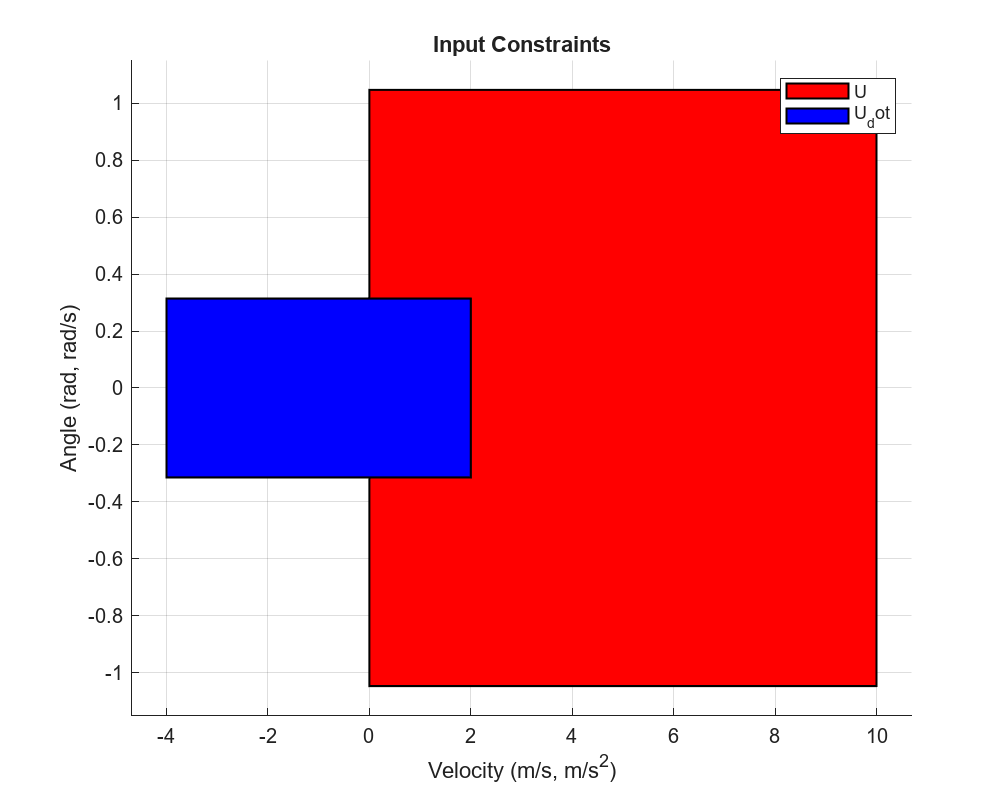
\includegraphics[width = 0.6 \columnwidth]{figs/input_constraints.png}
    \caption{Halfspace visualization of the input constraints.}\label{fig:inputConstraints}
\end{figure}

% Cost Function
\subsection{Cost Function}

The primary cost function will be linear from the system state as derived the cost map as the sum of the region that the vehicle would occupy.
An example is shown in \autoref{fig:occupancyMap}.

\begin{figure}[h]
    \centering
    
\includegraphics[width = 0.4\columnwidth]{figs/costmap1.png}
    \caption{An example occupancy map provided from the perception stack. The }\label{fig:occupancyMap}
\end{figure}

This is first done by directly converting the occupancy map of the vehicle in positions into a function of the system state, visualized in \autoref{fig:costMap}, as just $f_{map}(x_k)$.
Note that this is also normalized and the function itself is currently treated as a piecewise function (unfortunately causing issues within implementation).

\begin{figure}[h]
    \centering
    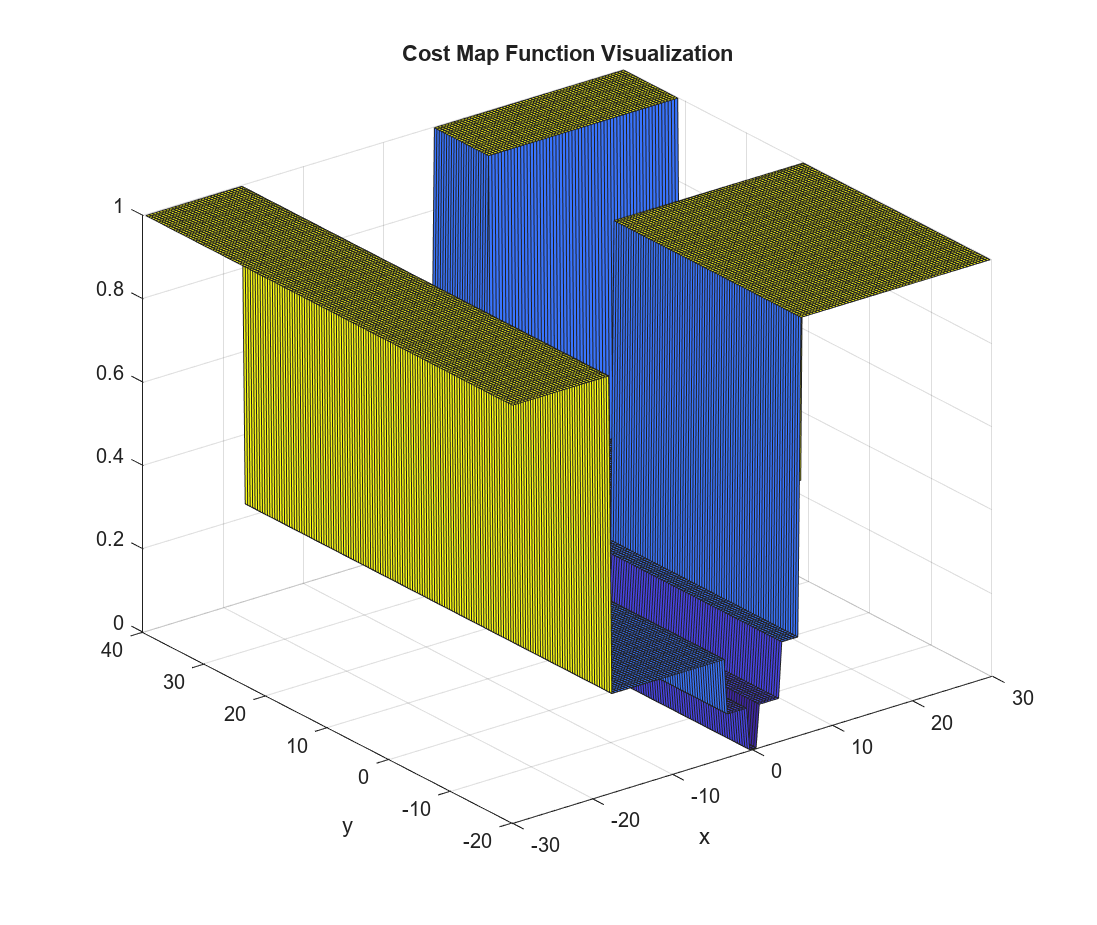
\includegraphics[width = 0.7 \columnwidth]{figs/surf_costmap1.png}
    \caption{An example cost map after converting into a direct function of system state and further interpolating.}\label{fig:costMap}
\end{figure}

Additionally, an objective will be included that describes the forward progression along a proposed route, $f_{progress}(x_k)$.

As was found out within actual implementation, the occupancy map was additionally simplified to a static function relative to the initial path for each time-step to remove the piecewise-nature or interpolation required by the full cost-map.

The results section will include simulation results for specific demonstrative cost-functions.
Note that in the results, the actual path is generated each time-step and the primary visualization as that which closes the loop and actually implements the desired inputs (i.e. actual MPC).
In the actual system, the PID would track the generated state-trajectory while the inputs are not explicitly used (i.e. similar to hieratical MPC).

% -----------------------------------------------------
% Simulation and Results
% -----------------------------------------------------
\section{Simulation and Results}\label{sec:sim_and_results}

The actual system was modeled MATLAB using multiple toolboxes (yalmip\cite{yalmip}, MPT3\cite{MPT3}, gurobi\cite{gurobi}, and IPOPT\cite{ipopt}).

Many simulations were run and the few included here are used to demonstrate the simpler operations.
The follwoing parameters were used within these results:
\begin{itemize}
    \item $N = 15$
    \item $\Delta t = 1$ [s]
    % \item Multiple $q(x_k,u_k)$ and $p(x_{n})$ tested
    \item $h_{u}(u_k) \leq 0$ 
    \item $h_{\dot{u}}(u_{k+1},u_{k-1}) = \frac{u_{k+1}-u_{k}}{\Delta t}\leq 0$
\end{itemize}
The simulations were ran with $T = 10$ [s] and the results for both fmincon and ipopt are provided.

\subsection{$90^\circ$ turn}
\subsubsection{Turn with optimal lane reference}
One success includes a 90 degree turn and just maximization of the distance in that direction. 
The specific cost function specified $f_{map} = (x_k - 0)^2 + (\theta_k - \pi/2)^2$ and $f_{progress} = -y_k$.
The closed loop trajectory for both fmincon and ipopt are similar, path compared in \autoref{fig:maxY_quiver_comp}, while the computation time is very different with 665 [s] and 85 [s] for fmincon and ipopt respectivly.
\begin{figure}[h]
    \centering
    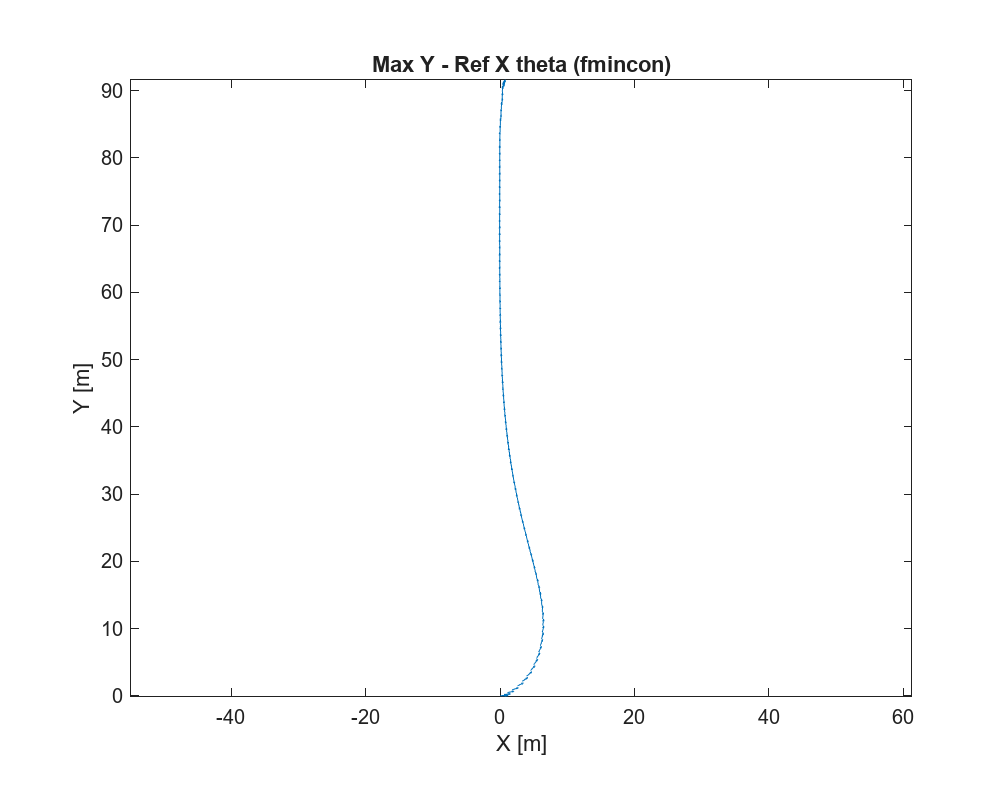
\includegraphics[width = 0.49\columnwidth]{figs/Max_Y_-_Ref_X_theta_(fmincon)_quiver.png}
    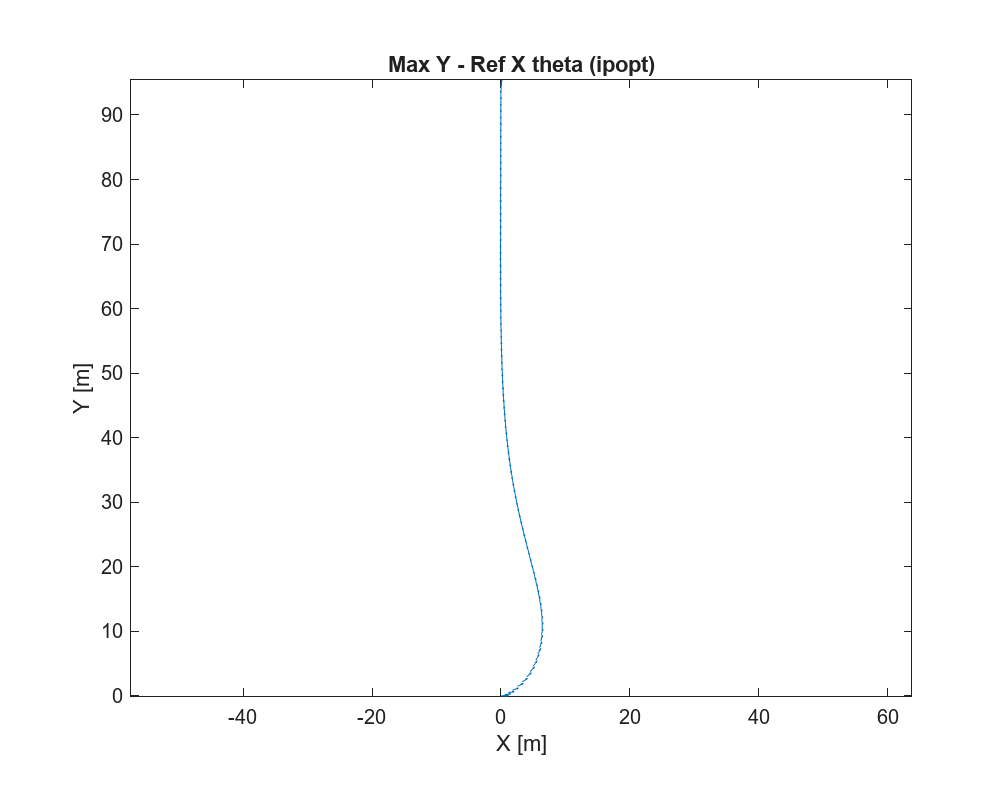
\includegraphics[width = 0.49\columnwidth]{figs/Max_Y_-_Ref_X_theta_(ipopt)_quiver.png}
    \caption{Quiver plot of the closed-loop simulation for $J_k = -y_k + (x_k - 0)^2 + (\theta_k - \pi/2)^2$ using fmincon (left) and ipopt (right).}\label{fig:maxY_quiver_comp}
\end{figure}

The plot of the state and input trajectories for the ipopt simulation is shown in \autoref{fig:maxY_ipopt}.
As can be seen, the input is well planned to turn as much as possible at first and then optimize for distance in the Y direction by having an overdamped response for returning to the center of the plot.
\begin{figure}[h]
    \centering
    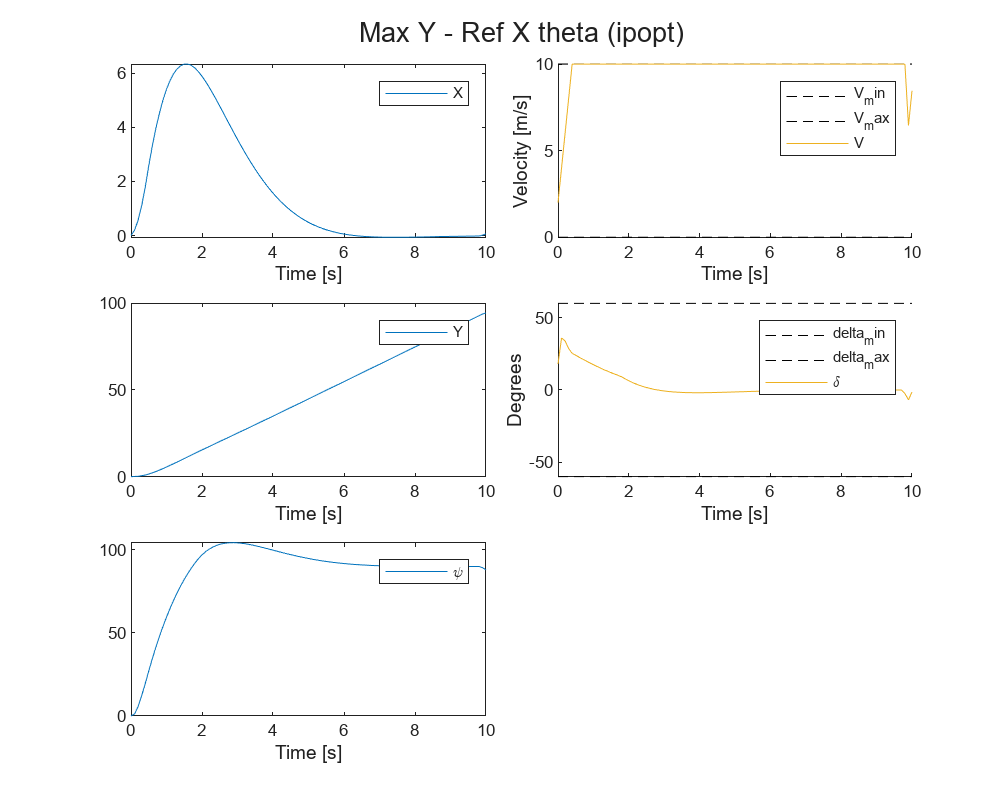
\includegraphics[width = \columnwidth]{figs/Max_Y_-_Ref_X_theta_(ipopt)_traj.png}
    \caption{Closed loop simulation to maximize the Y position with $J_k = -y_k + (x_k - 0)^2 + (\theta_k - \pi/2)^2$ using ipopt.}\label{fig:maxY_ipopt}
\end{figure}
The fmincon version is attached in the Appendix as \autoref{fig:maxY_fmincon}.

\subsubsection{Removing the cost map term}
When testing the ability for the controller to operate with solely an unstructured ``go as far that direction'', i.e. maximize in the y-direction ($f_{progress} = -y_N$) at the final time-step.
The fmincon solution was effective in its goal while the ipopt solution would be classified as a failure.
The path comparison can be seen in \autoref{fig:maxY_final_quiver_comp}. 

\begin{figure}[h]
    \centering
    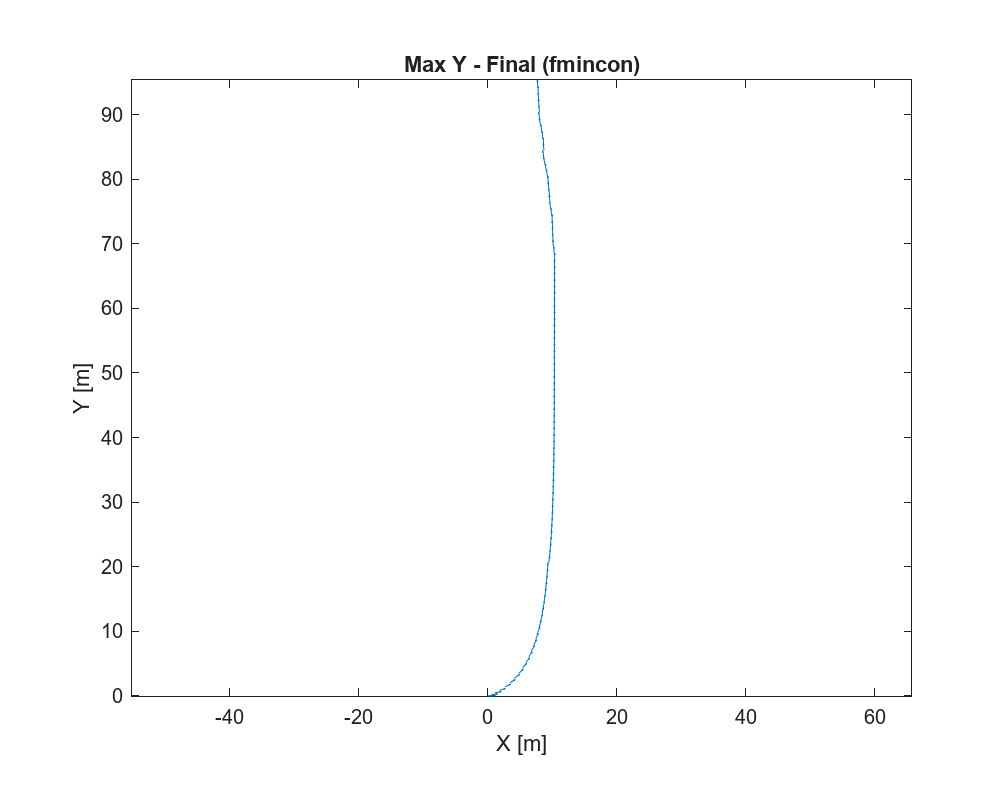
\includegraphics[width = 0.49\columnwidth]{figs/Max_Y_-_Final_(fmincon)_quiver.png}
    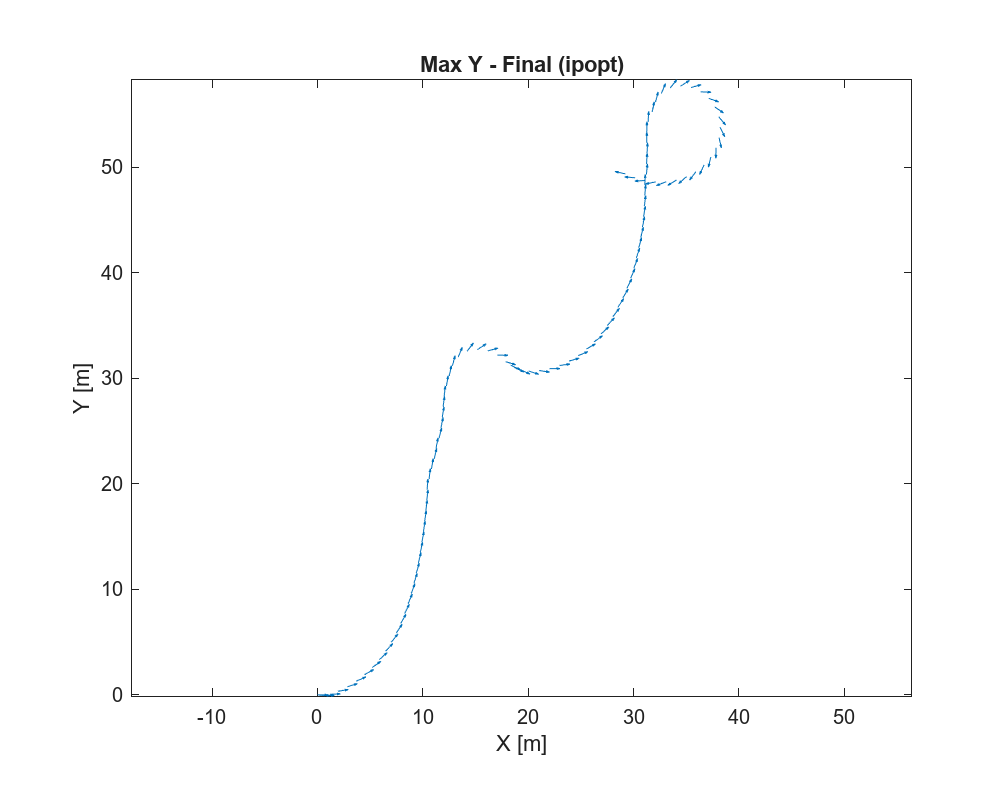
\includegraphics[width = 0.49\columnwidth]{figs/Max_Y_-_Final_(ipopt)_quiver.png}
    \caption{Quiver plot of the closed-loop simulation for $J = y_N$ using fmincon (left) and ipopt (right).}\label{fig:maxY_final_quiver_comp}
\end{figure}

When looking into the simulation in more detail, it is clear that the fmincon,shown in \autoref{fig:maxY_final_fmincon}, followed a similar trajectory as when the cost map component was included, with the biggest difference being that it does not return to the center within the $x$ direction.

\begin{figure}[h]
    \centering
    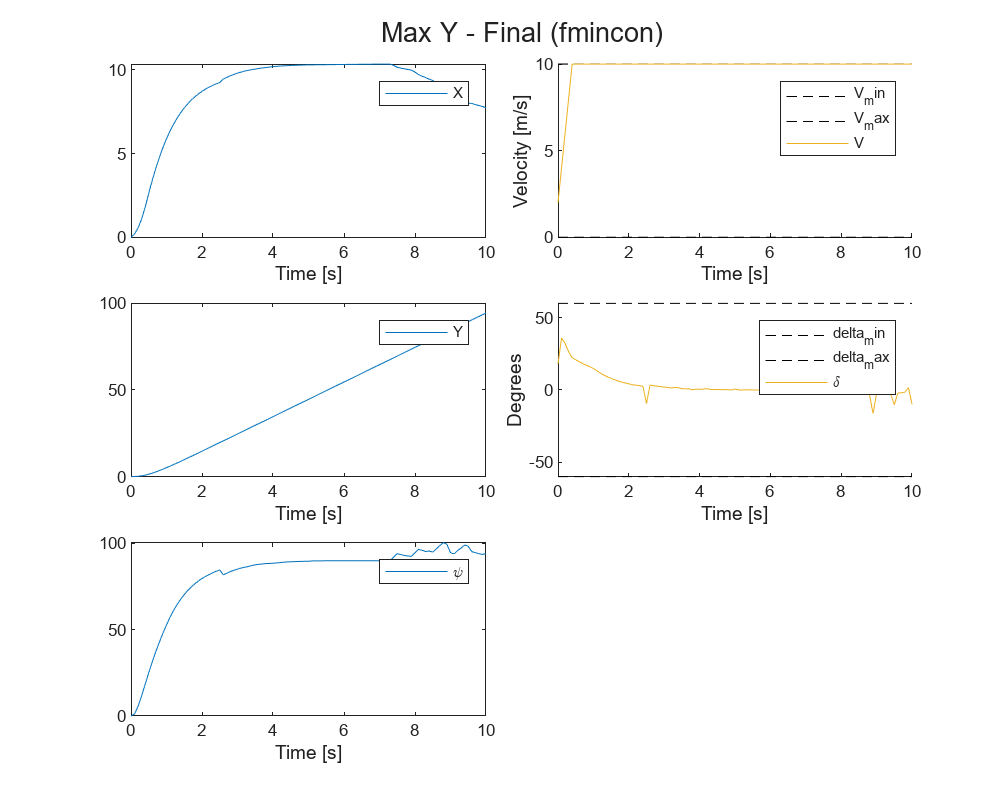
\includegraphics[width = \columnwidth]{figs/Max_Y_-_Final_(fmincon)_traj.png}
    \caption{Closed loop simulation to maximize the Y position with $J_N = -y_N$ using fmincon.}\label{fig:maxY_final_fmincon}
\end{figure}

The results for the ipopt solver, shown in \autoref{fig:maxY_final_ipopt}, is more interesting and certainly classified as a ``failure''.
Although forward progress made, the vehicle appears to get up to speed as quickly as possible than makes a small mistake in turning until eventually having to correct, over-correct, and then do a donut to hopefully get going in the correct direction again.

\begin{figure}[h]
    \centering
    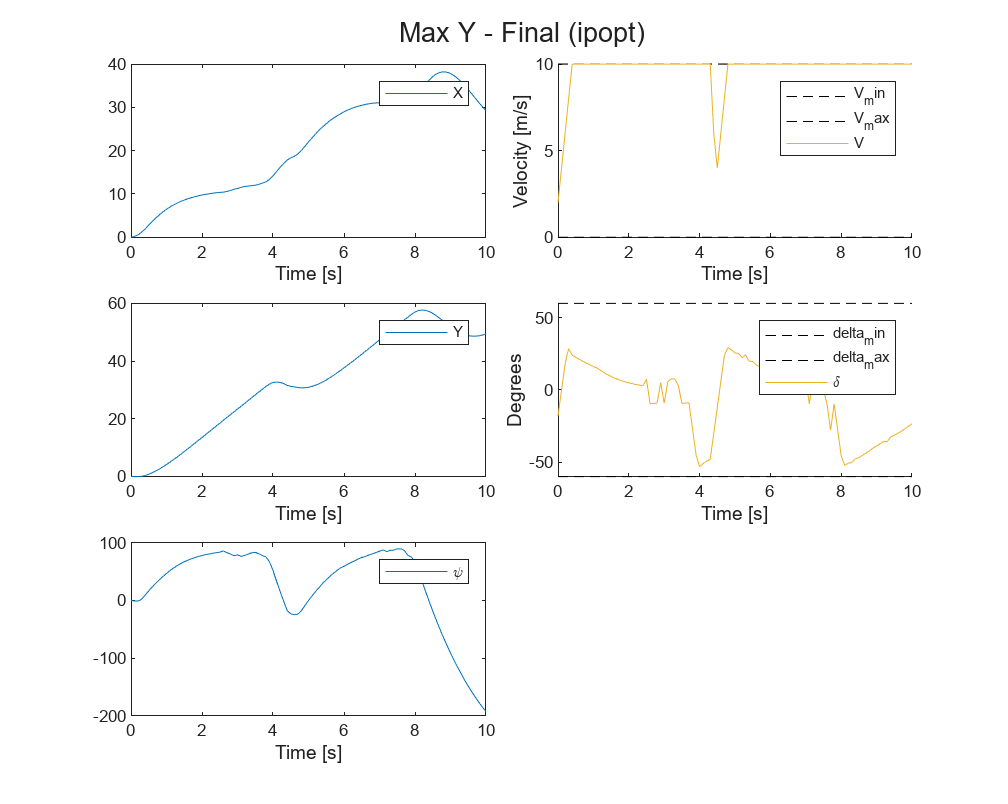
\includegraphics[width = \columnwidth]{figs/Max_Y_-_Final_(ipopt)_traj.png}
    \caption{Closed loop simulation to maximize the Y position with $J_N = -y_N$ using ipopt.}\label{fig:maxY_final_ipopt}
\end{figure}

\subsection{U-turn}
When testing a more complicated case, such as a U-turn, produced even more interesting results.

\subsubsection{Unstructured turn around}
Implementation with only the $f_{progress}$ term, resulted in different turning behaviors requiring overcorrection for both solvers as seen in \autoref{fig:minX_final_quiver_comp}.
\begin{figure}[h]
    \centering
    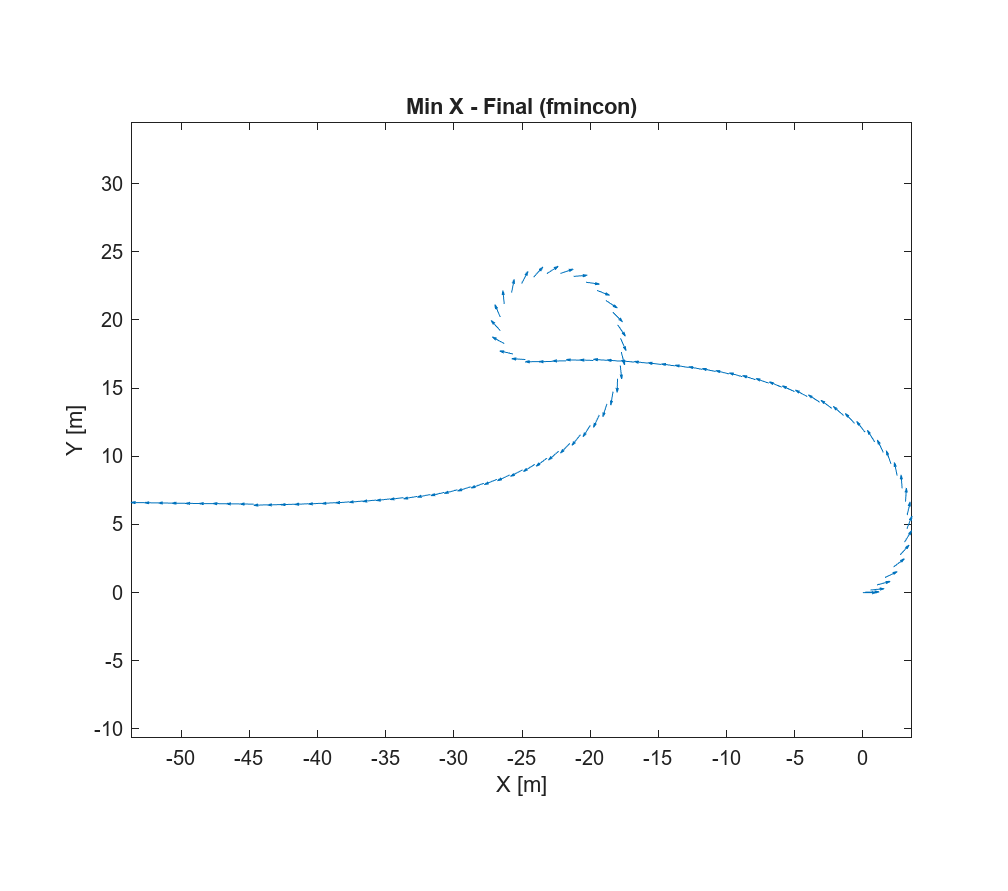
\includegraphics[width = 0.49\columnwidth]{figs/Min_X_-_Final_(fmincon)_quiver.png}
    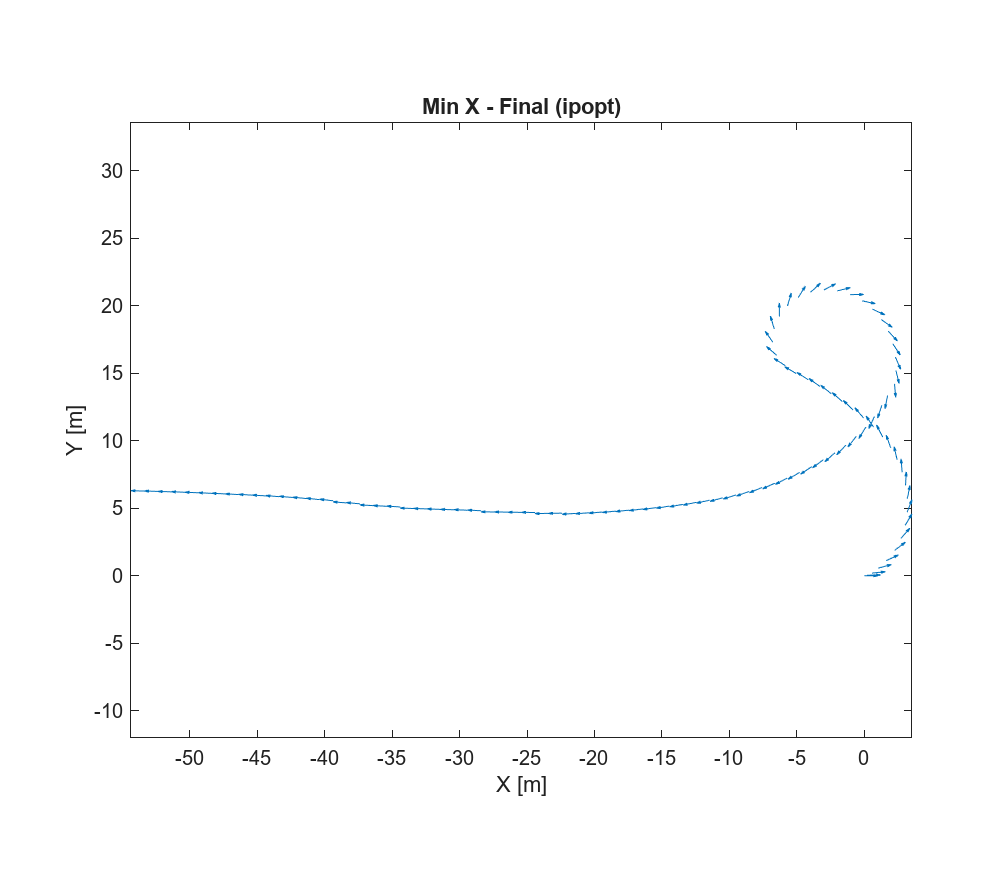
\includegraphics[width = 0.49\columnwidth]{figs/Min_X_-_Final_(ipopt)_quiver.png}
    \caption{Quiver plot of the closed-loop simulation for $J = x_N$ using fmincon (left) and ipopt (right).}\label{fig:minX_final_quiver_comp}
\end{figure}
When looking at the trajectories in more detail, shown in \autoref{fig:minX_final_both} in the appendix, the general shape of the response (turning, under correction, overcorrection, and donut) is similar but with different delays in response.

\subsubsection{Cost-map term included}
Implementation of the U-turn with a cost-map term, $f_{map} = (y_k-0)^2/100 + (\theta_k - \pi)^2$, was successful for the ipopt case as seen in \autoref{fig:Min_X_with_special_ref_ipopt}; however not so for the fmincon case (\autoref{fig:Min_X_with_special_ref_fmincon} shown in appendix) as it ended up with way too many overcorrection turns.
\begin{figure}[h]
    \centering
    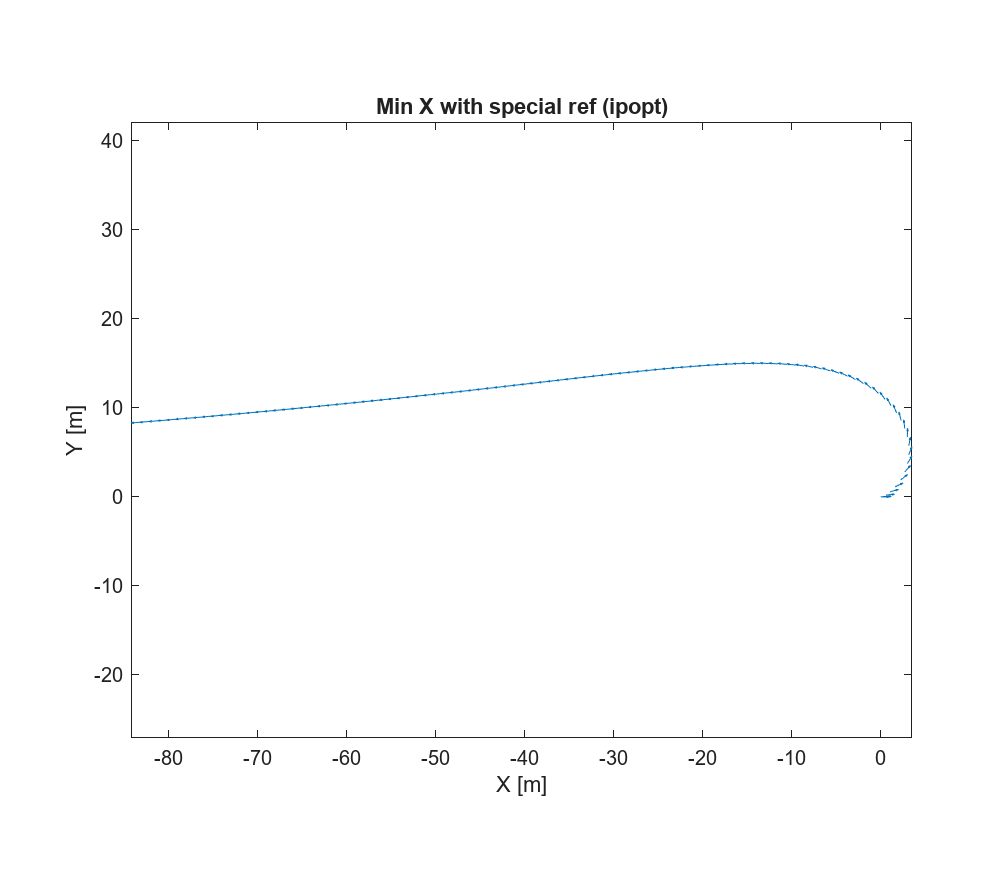
\includegraphics[width = 0.45\columnwidth]{figs/Min_X_with_special_ref_(ipopt)_quiver.png}
    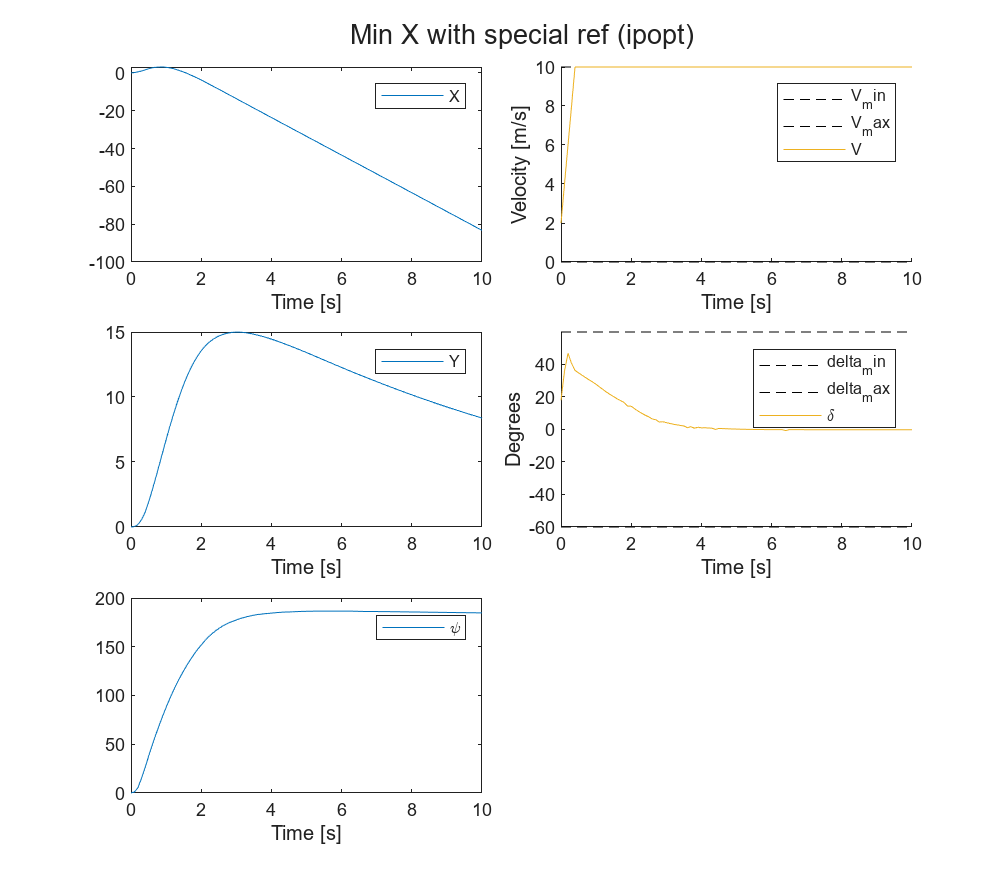
\includegraphics[width = \columnwidth]{figs/Min_X_with_special_ref_(ipopt)_traj.png}	
    \caption{Closed loop simulation with $f_{map} = (y_k-0)^2/100 + (\theta_k - \pi)^2$ using ipopt.}\label{fig:Min_X_with_special_ref_ipopt}
\end{figure}
An interesting note about the $f_{map}$ term is that if the cost map function ends up being a reference to $-180^\circ$ instead of $+180^\circ$, $f_{map} = (y_k-0)^2/100 + (\theta_k + \pi)^2$, then the vehicle would do the U-turn in the other direction.

% -----------------------------------------------------
% Conclusion
% -----------------------------------------------------
\section{Conclusion}
The biggest conclusion from this project is that that current nonlinear MPC setup is not a feasible solution for NOVA to do path planning, even in the case for just generating training data for the neural network.
It was found that it is possible to create specific $f_{map}$ functions that could be effective; however the creation of these from the discrete values provided from the perception stack would be difficult to create with no gaurentee that it may work.

Additionally, this project was a major demonstration of how using different optimization solvers can have a major impact on the computation time, but also the results themselves.
A rough testing comparison of the different testing times is included in \autoref{tbl:optSolverComp} and clearly IPOPT was far faster in every test, but even so it is not nearly fast enough to generate a lot of training data let alone for online operation.

\begin{table}[h]
    \centering
    \caption{Computation time comparison between FMINCON and IPOPT}\label{tbl:optSolverComp}
    \begin{tabular}{|l|l|l|}
		\hline
		\textbf{}                       & \textbf{FMINCON} & \textbf{IPOPT}  \\ \hline
		Min Y - Unstructured            & 243.79           & 164.75          \\ \hline
		Min Y - Final                   & 235.91           & 155.6           \\ \hline
		Min Y - Ref X and theta         & 438.67           & 71.79           \\ \hline
		\textbf{Min X - Final}          & \textbf{1077.6}  & \textbf{164.58} \\ \hline
		Min X with +180                 & 395.71           & 191.69          \\ \hline
		\textbf{Min X with special ref} & \textbf{344.52}  & \textbf{165.16} \\ \hline
		\textbf{Max Y - Final}          & \textbf{331.71}  & \textbf{140.49} \\ \hline
		\textbf{Max Y - Ref X theta}    & \textbf{665.82}  & \textbf{85.492} \\ \hline
    \end{tabular}
\end{table}


% % -----------------------------------------------------
% % Aknowledgements
% % -----------------------------------------------------
% \section*{Acknowledgements}
% \begin{center}
%     
\includegraphics[width=0.25\columnwidth]{figs/NOVA-logo.png}\\
%     Research Advisor: Justin Ruths\\
%     Course Professor: Justin Koeln
% \end{center}

% -----------------------------------------------------
% References
% -----------------------------------------------------
\bibliography{refs}{} 
\bibliographystyle{IEEEtran}

% \newpage
\appendix
\section*{Github}
See my github repo for this project for all the source code and additional results: 
\url{https://github.com/jonaswagner2826/MECH6V29_MPC_FinalProject}

\section*{Matlab results}\label{apx:MATLAB}
MATLAB code is included in submission.

\section*{Additional Results}
\begin{figure}[h]
    \centering
    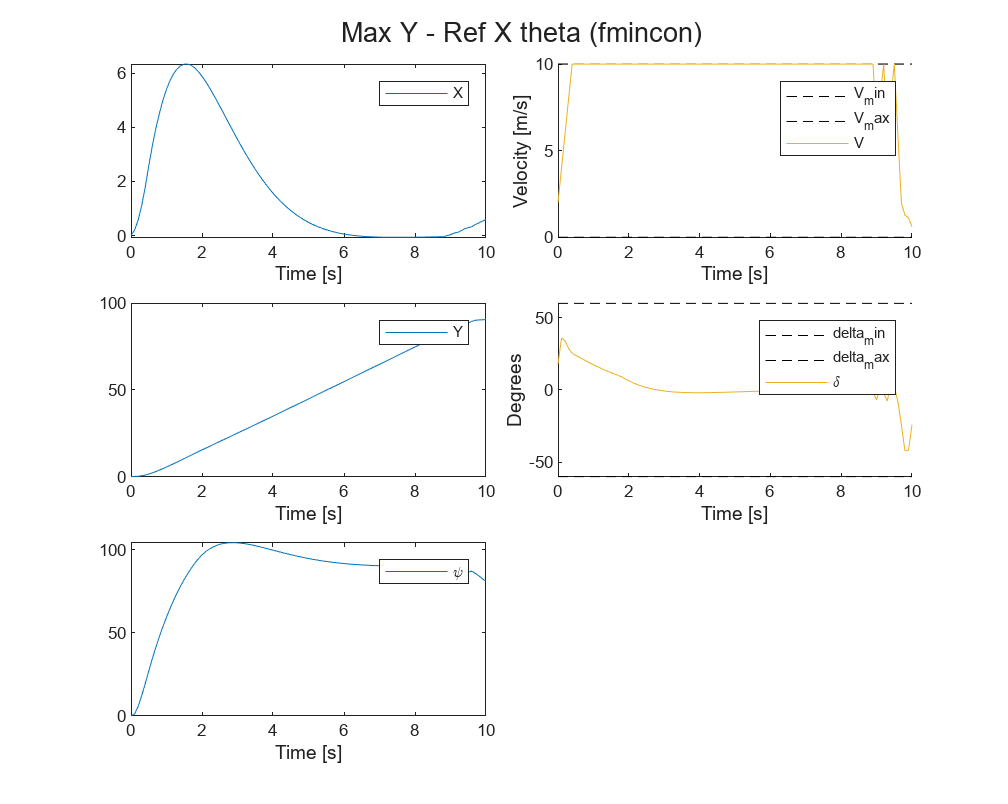
\includegraphics[width = \columnwidth]{figs/Max_Y_-_Ref_X_theta_(fmincon)_traj.png}
    \caption{Closed loop simulation to maximize the Y position with $J_k = -y_k + (x_k - 0)^2 + (\theta_k - \pi/2)^2$ using fmincon.}\label{fig:maxY_fmincon}
\end{figure}

\begin{figure}[h]
    \centering
    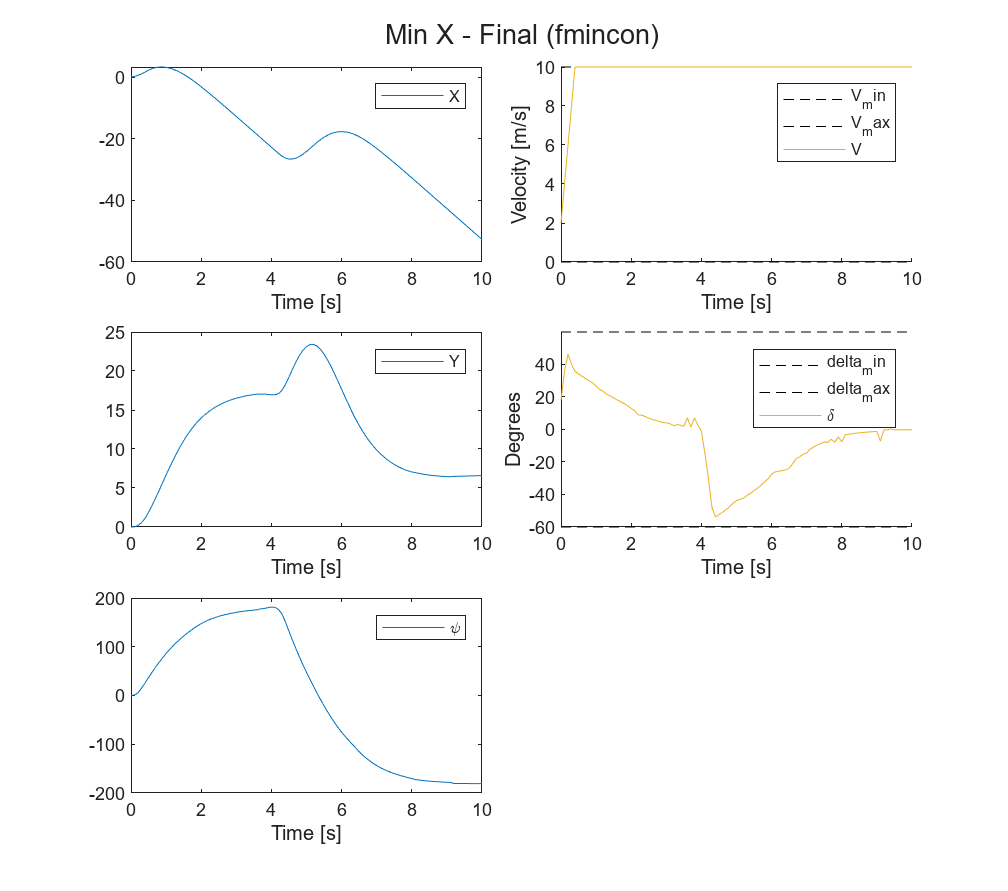
\includegraphics[width = \columnwidth]{figs/Min_X_-_Final_(fmincon)_traj.png}
    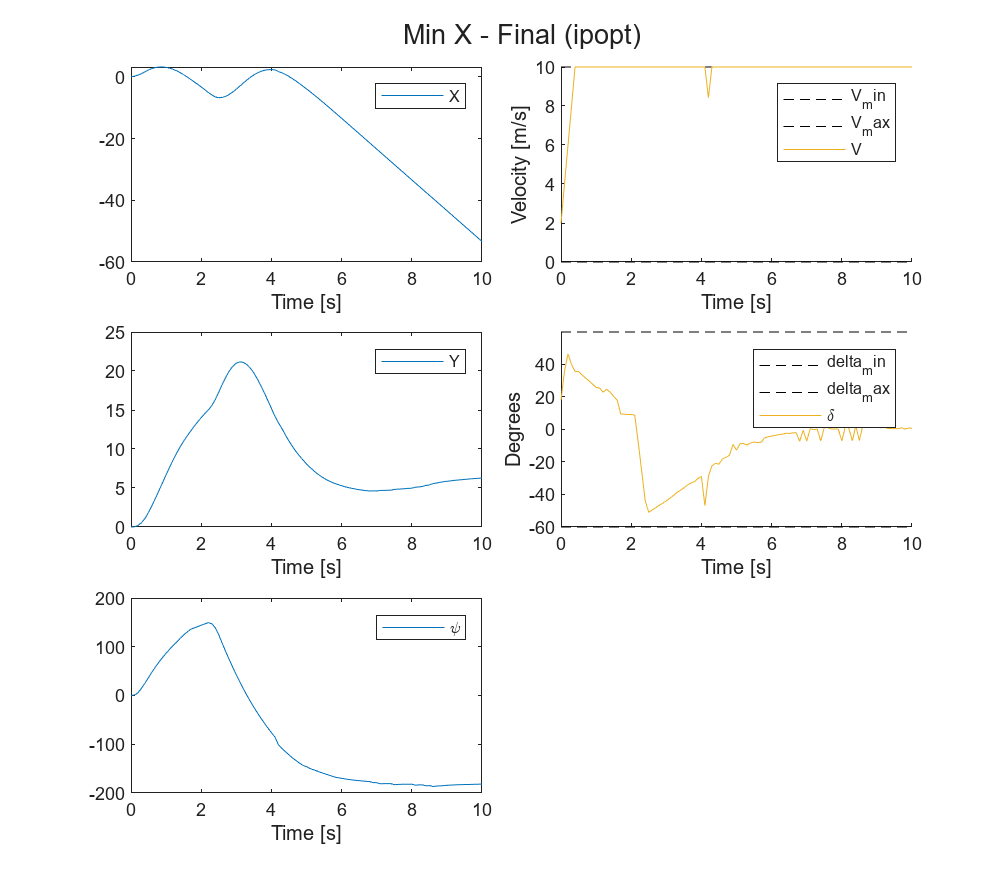
\includegraphics[width = \columnwidth]{figs/Min_X_-_Final_(ipopt)_traj.png}
    \caption{Closed loop simulation to maximize the Y position with $J_N = x_N$ using fmincon(top) and ipopt (bottom).}\label{fig:minX_final_both}
\end{figure}

\begin{figure}
    \centering
    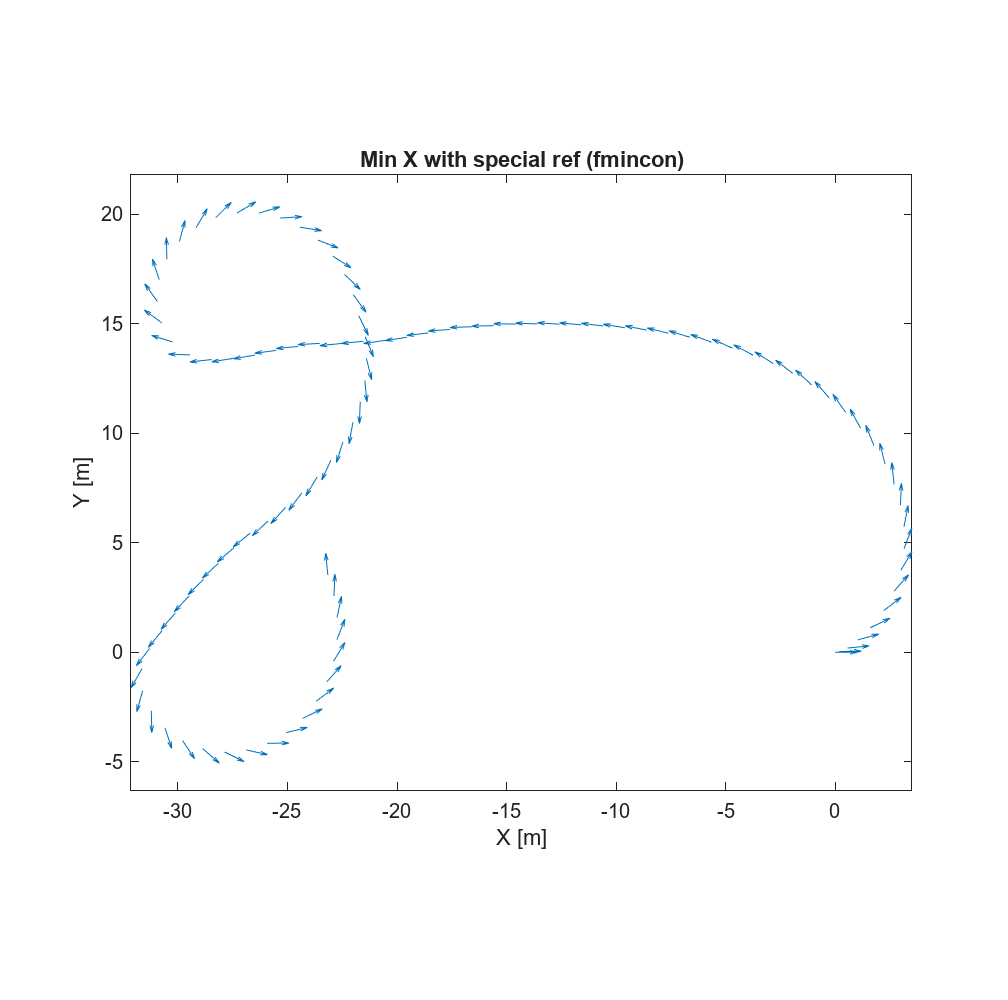
\includegraphics[width = 0.49\columnwidth]{figs/Min_X_with_special_ref_(fmincon)_quiver.png}
    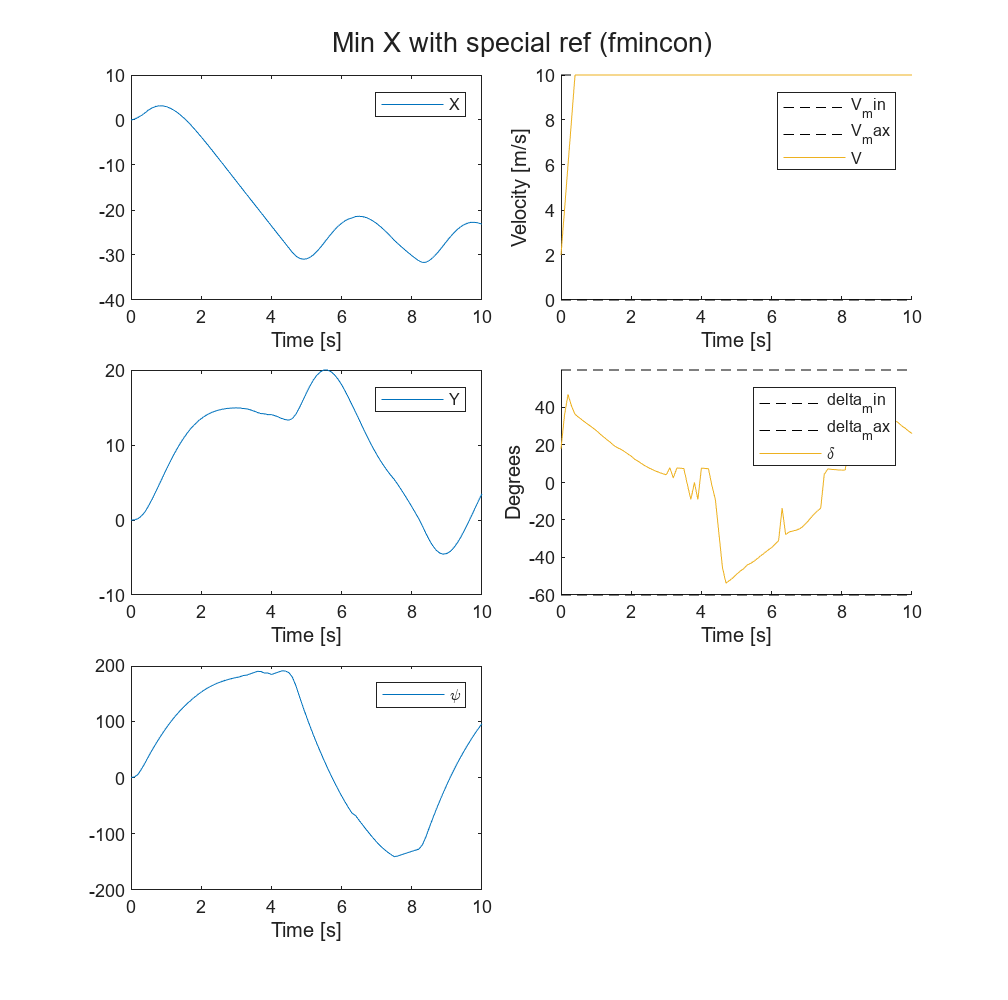
\includegraphics[width = \columnwidth]{figs/Min_X_with_special_ref_(fmincon)_traj.png}	
    \caption{``Failed'' fmincon case for the cost-map term version of a U-turn}\label{fig:Min_X_with_special_ref_fmincon}
\end{figure}

\end{document}
